\documentclass[../DS01.tex]{subfiles}%
\graphicspath{{./figures/}}%

\begin{document}%

% \section[35\footnotesize$\times$\num{1.5}]"P"{Formation d'un arc-en-ciel\ifcorrige{~\small\textit{(D'après banque PT 2024)}}}
\section[51]"P"{Formation d'un arc-en-ciel\ifcorrige{~\small\textit{(D'après banque PT 2024)}}}

\enonce{%
	Lorsque le beau temps revient juste après une averse, on observe parfois la
	formation d'un arc-en-ciel à l'horizon. Il s'agit d'un phénomène optique de
	dispersion de la lumière solaire, qui se réfracte et se réfléchit dans des
	gouttelettes d'eau en suspension dans l'air. La première théorie permettant
	d'expliquer ce phénomène a été établie par Descartes en 1637 à l'aide des lois
	de la réflexion et de la réfraction. Il mit en évidence qu'un-e
	observateur-ice situé-e au niveau du sol reçoit un faisceau de rayons émergents
	correspondant au maximum de l'angle de déviation des gouttelettes d'eau. Comme
	celui-ci dépend de la longueur d'onde des rayons lumineux, on peut ainsi
	observer la dispersion de la lumière solaire. Dans cette partie, nous allons
	mettre en évidence les principaux résultats de cette théorie.

	\begin{tcb}[blankest, sidebyside](null){}
		On considère un rayon lumineux monochromatique issu du Soleil $S$, qui arrive
		sur une gouttelette d'eau sphérique en suspension dans l'air sous un angle
		d'incidence $i_1$, comme représenté sur la Figure~\ref{fig:arc_plain}. Après
		une première réfraction, une réflexion et une seconde réfraction, le rayon
		émerge de la gouttelette sous un angle de réfraction $i_4$. Il se dirige alors
		vers un-e observateur-ice $O$ situé-e au niveau du sol. On suppose que l'air
		est un milieu d'indice optique égal à 1, et on note $n$ l'indice optique de
		l'eau.
		\bigbreak
		L'orientation des différents angles à chaque interface est définie sur la
		Figure~\ref{fig:arc_plain}, et on définit positivement les angles orientés
		dans le sens trigonométrique.
		\tcblower
		\begin{center}
			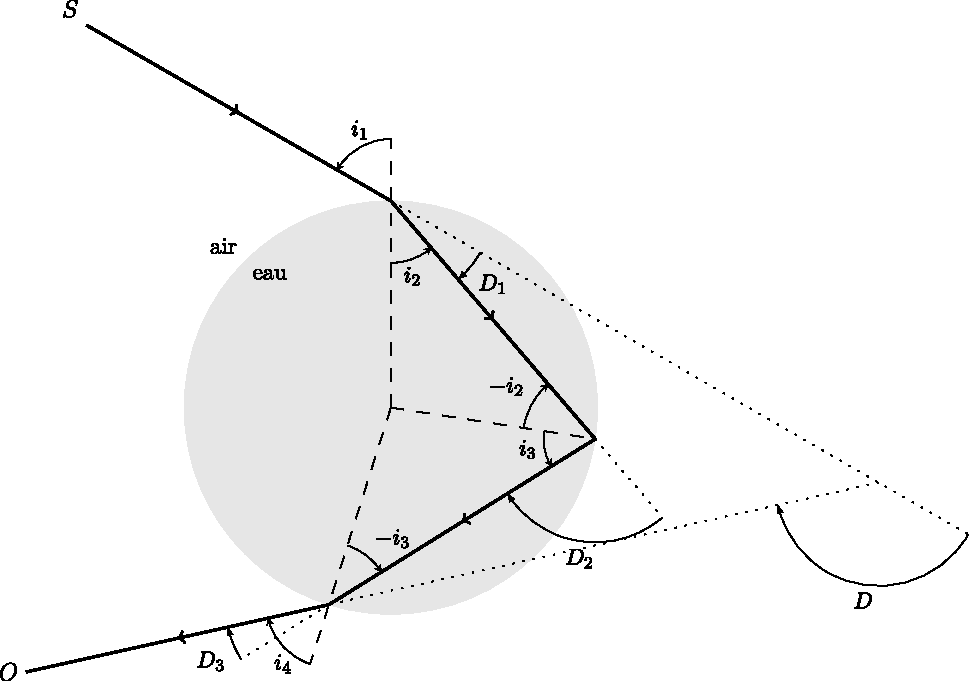
\includegraphics[width=\linewidth]{arc_plain}
			\captionof{figure}{Trajet d'un rayon lumineux dans une gouttelette d'eau
				sphérique en suspension dans l'air.}
			\label{fig:arc_plain}
		\end{center}
	\end{tcb}

	% On considère un rayon lumineux monochromatique issu du Soleil $S$, qui arrive
	% sur une gouttelette d'eau sphérique en suspension dans l'air sous un angle
	% d'incidence $i_1$, comme représenté sur la Figure~\ref{fig:arc_plain}. Après
	% une première réfraction, une réflexion et une seconde réfraction, le rayon
	% émerge de la gouttelette sous un angle de réfraction $i_4$. Il se dirige alors
	% vers un-e observateur-ice $O$ situé-e au niveau du sol. On suppose que l'air
	% est un milieu d'indice optique égal à 1, et on note $n$ l'indice optique de
	% l'eau.
	% \begin{center}
	% 	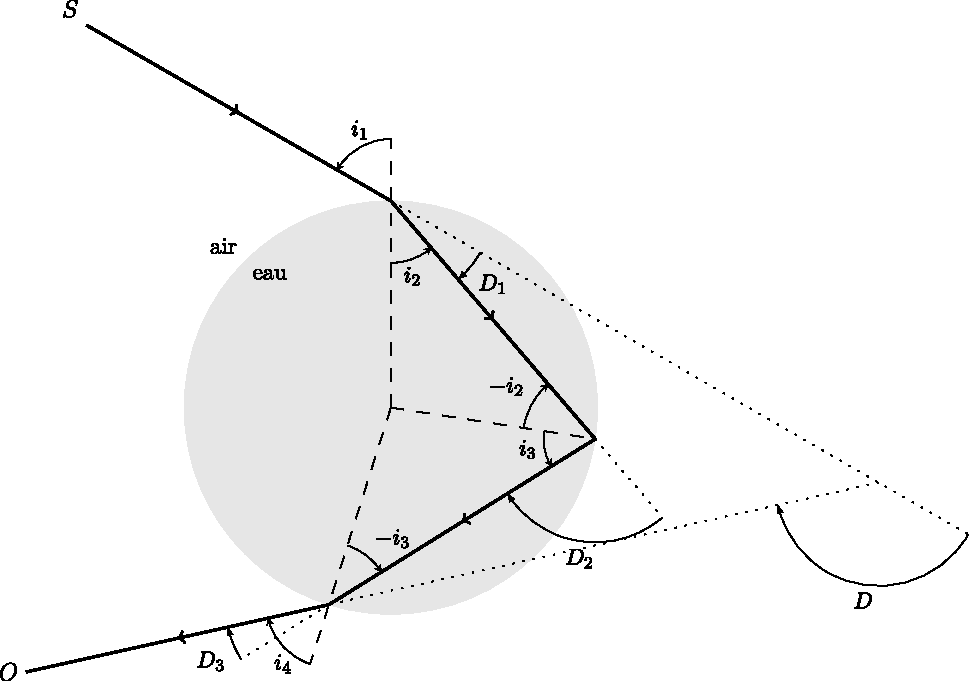
\includegraphics[width=\linewidth]{arc_plain}
	% 	\captionof{figure}{Trajet d'un rayon lumineux dans une gouttelette d'eau
	% 		sphérique en suspension dans l'air.}
	% 	\label{fig:arc_plain}
	% \end{center}
	% L'orientation des différents angles à chaque interface est définie sur la
	% Figure~\ref{fig:arc_plain}, et on définit positivement les angles orientés
	% dans le sens trigonométrique.
}%

\QR[3]{%
	Exprimer les angles de déviation $D_1$, $D_2$ et $D_3$ à chaque interface et
	en fonction de $i_1$, $i_2$, $i_3$ et $i_4$, en tenant compte de l'orientation
	de ces angles.
}{%
	On lit sur la figure~:
	\begin{gather*}
		i_2 - D_1 = i_1
		\qquad
		-(-i_2) + i_3 - D_2 = \pi
		\qquad
		D_3 + (-i_3) = i_4
		\\\Lra
		\boxed{D_1 \stm[-1]{=} i_2-i_1}
		\qquad
		\boxed{D_2 \stm[-1]{=} i_2 + i_3 - \pi}
		\qquad
		\boxed{D_3 \stm[-1]{=} i_3+i_4}
	\end{gather*}
}%

\QR[4]{%
	À l'aide des lois de \textsc{Snell-Descartes}, exprimer les angles $i_2$,
	$i_3$ et $i_4$ en fonction de $i_1$ et $n$.
}{%
	D'après la loi de la réfraction,
	\begin{gather*}
		1 \times \sin(i_1) \stm{=} n \sin(i_2)
		\Lra
		\boxed{i_2 \stm{=} \arcsin(\frac{\sin(i_1)}{n})}
	\end{gather*}
	D'après la loi de la réflexion,
	\begin{gather*}
		i_3 \stm{=} i_2 = \arcsin(\frac{\sin(i_1)}{n})
	\end{gather*}
	Enfin, d'après la loi de la réfraction encore,
	\begin{gather*}
		\sin(i_4) = n \sin(-i_3) = -n\sin(i_2) = -\sin(i_1)
		\\\Lra
		\boxed{i_4 \stm{=} -i_1}
	\end{gather*}
}%

\QR[2]{%
	En déduire que l'angle de déviation totale $D$ peut s'exprimer~:
	\[
		D = 4 \arcsin(\frac{\sin(i_1)}{n}) - 2i_1 - \pi
	\]
}{%
	La déviation totale s'écrit
	\begin{align*}
		D         & \stm{=} D_1+D_2+D_3
		\\\Lra
		D         & = (i_2 - i_1) + (i_2 + i_3 - \pi) + (i_4 + i_3)
		\\\Lra
		D         & = -i_1 + 2i_2 + 2i_3 + i_4 - \pi
		\\\Lra
		\Aboxed{D & \stm{=} 4 \arcsin(\frac{\sin(i_1)}{n}) - 2i_1 - \pi}
	\end{align*}
}%

\enonce{%
	\begin{tcb}[blankest, sidebyside](null){}
		On représente l'évolution de $D$ en fonction de $i_1$ sur la
		Figure~\ref{fig:Di1}, en prenant $n = \num{1.33}$ pour l'indice optique de
		l'eau. L'angle de déviation présente un maximum $D\ind{max}$ pour un certain
		angle d'indicence $i_{1,\rm max}$ qui correspond au faisceau de rayons
		émergents reçu par l'observateur-ice.
		\bigbreak
		On rappelle que la dérivée de la fonction trigonométrique $f(x) = \arcsin(x)$
		s'exprime~:
		\[
			\dv{f}{x} = \frac{1}{\sqrt{1-x^2}}
		\]
		\tcblower
		\begin{center}
			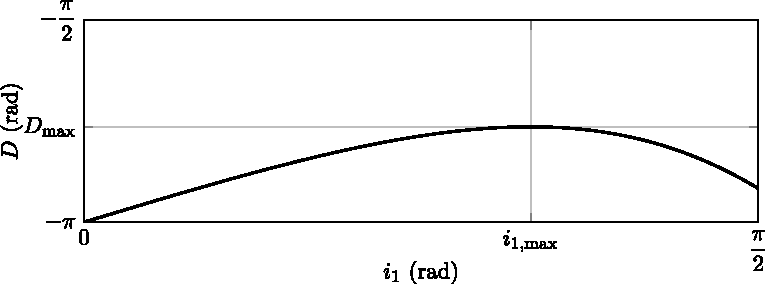
\includegraphics[width=\linewidth]{Di1}
			\captionof{figure}{Évolution de l'angle de déviation $D$ en fonction de l'angle
				d'incidence $i_1$.}
			\label{fig:Di1}
		\end{center}
	\end{tcb}
}%

\QR[8]{%
	Montrer que l'angle d'incidence $i_{1,\rm max}$ vérifie l'équation suivante~:
	\[
		\sin(i_{1,\rm max}) = \sqrt{\frac{4-n^2}{3}}
	\]
}{%
	Posons $x = \sin(i_1)$. Alors,
	\begin{DispWithArrows*}[]
		D(x) &\stm{=}
		4 \arcsin{\frac{x}{n}} - 2\arcsin{x} - \pi
		\Arrow{On dérive}
		\\\Ra
		\dv{D}{x} &\stm{\stm(un){=}}
		4\times \frac{1}{n} \frac{1}{\sqrt{1-\dfrac{x^2}{n^2}}} -
		\frac{2}{\sqrt{1-x^2}}
	\end{DispWithArrows*}
	Cette dérivée s'annule au niveau du maximum, c'est-à-dire
	\begin{align*}
		\frac{4}{n} \frac{1}{\sqrt{1-\dfrac{x\ind{max}^2}{n^2}}}   & \stm{=}
		\frac{2}{\sqrt{1-x\ind{max}^2}}
		\\\Lra
		\frac{n^2}{16} \left( 1 - \frac{x\ind{max}^2}{n^2} \right) & \stm{=}
		\frac{1-x\ind{max}^2}{4}
		\\\Lra
		n^2-x\ind{max}^2                                           & \stm{=}
		4 - 4x\ind{max}^2
		\\\Lra
		3x\ind{max}^2                                              & \stm{=}
		4-n^2
		\\\Lra
		\Aboxed{\sin(i_{1,\rm max})                                & \stm{=} \sqrt{\frac{4-n^2}{3}}}
	\end{align*}
}%

\QR[2]{%
	En déduire l'expression du maximum $D\ind{max}$ en fonction de $n$.
}{%
	On injecte cette valeur dans l'expression de $D$~:
	\[
		\boxed{
			D\ind{max} \stm{\stm(un){=}}
			4 \arcsin(\frac{1}{n}\sqrt{\frac{4-n^2}{3}}) -
			2\arcsin{\sqrt{\frac{4-n^2}{3}}} - \pi
		}
	\]
}%

\enonce{%
	\begin{tcb}[blankest, sidebyside](null){}
		On représente l'évolution de $D\ind{max}$ en fonction de $n$ sur la
		Figure~\ref{fig:DmaxN}, pour $1 \leq n \leq 2$.
		\smallbreak
		L'eau étant un milieu dispersif, son indice optique $n$ dépend de la
		longueur d'onde $\lambda$ du rayon lumineux considéré. En 1836,
		\textsc{Cauchy} établit que l'indice optique d'un tel milieu peut s'exprimer
		sous la forme~:
		\[
			n(\lambda) = A + \frac{B}{\lambda^2}
		\]
		avec $A$ et $B$ des constantes positives, caractéristiques du milieu.
		\tcblower
		\begin{center}
			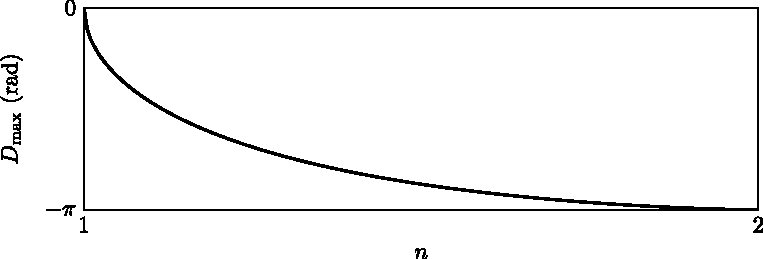
\includegraphics[width=\linewidth]{DmaxN}
			\captionof{figure}{Évolution du maximum $D\ind{max}$ en fonction de
				l'indice optique $n$.}
			\label{fig:DmaxN}
		\end{center}
	\end{tcb}

}%

\QR[2]{%
	Comment évolue le maximum $D\ind{max}$ lorsque la longueur d'onde $\lambda$
	augmente~? Justifier votre raisonnement.
}{%
	Si la longueur d'onde augmente, alors d'après la loi de \textsc{Cauchy}
	l'indice diminue \pt{1}, et d'après la courbe représentée l'angle de déviation
	maximale \textbf{augmente}. \pt{1}
}%

\QR[1]{%
	Rappeler l'intervalle de longueur d'onde constituant le spectre visible.
}{%
	Le spectre visible contient les longueurs d'ondes comprises entre
	$\SIrange{400}{800}{nm}$. \pt{1}
}%

\QR[8]{%
	Lorsque l'observateur-ice $O$ situé-e au niveau du sol regarde l'arc-en-ciel,
	aperçoit-iel l'anneau rouge situé au-dessus ou en-dessous de l'anneau violet~?
	Justifier votre raisonnement. Un schéma est attendu.
}{%
	La lumière atteint les gouttes avec toutes les incidences possibles, mais la
	courbe de déviation étant plus plate au voisinage du maximum, il y a le plus
	d'\textbf{intensité lumineuse} en sortie de la goutte dans la direction donnée
	par le \textbf{maximum de déviation}. On peut dire qu'il y a accumulation de
	lumière dans cette direction. \pt{1} + \pt{1}

	Compte tenu de ce qui précède, l'angle de déviation maximale est plus grand
	pour le rouge que pour le violet, \textbf{mais} comme l'angle de déviation est
	négatif, alors en valeur absolue
	\[
		\abs{D\ind{violet}} \stm{>} \abs{D\ind{rouge}}
	\]
	Autrement dit, l'angle entre les rayons entrant et sortant de la goutte, égal
	à $2\pi - \abs{D}$, est plus grand pour le rouge que pour le violet. \pt{1}

	Les rayons du Soleil arrivent tous parallèles les uns aux autres, pour une
	goutte donnée le rayon rouge part donc davantage vers le bas que le rayon
	violet. Cependant, les rayons «~qui comptent~» sont ceux qui aboutissent à
	l'œil de l'observateur-ice… qui ne sont pas déviés par la même goutte~! Comme
	le montre la Figure~\ref{fig:devarc}, les rayons rouges atteignant l'œil de
	l'observateur sont déviés par une goutte située plus haut \pt{1} que celle qui
	dévie les rayons violets. Ainsi, l'\textbf{anneau rouge paraît au dessus de
		l'anneau violet} dans le ciel. \pt{1}

	\begin{figure}[htbp!]
		\centering
		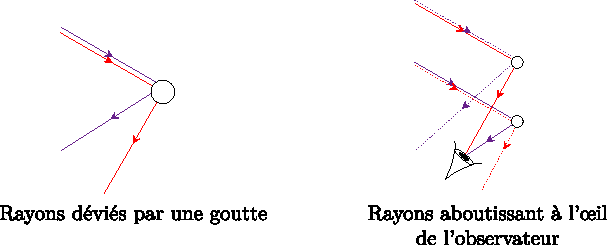
\includegraphics[scale=1]{devarc}
		\caption{Déviation des rayons et formation d'un arc-en-ciel.
			\protect \pt{1} + \protect \pt{1}}
		\label{fig:devarc}
	\end{figure}
}%

\enonce{%
	Lorsque les conditions d'observation sont excellentes, il est possible
	d'apercevoir un second arc-en-ciel dans le ciel, situé au-dessus de
	l'arc-en-ciel précédemment étudié. Il est même possible d'observer, dans de
	très rares occasions, un troisième arc-en-ciel qui s'ajoute aux deux
	précédents.
}%

\QR[4]{%
	En considérant toujours des gouttelettes d'eau sphériques en suspension dans
	l'air, expliquer l'origine de ces différents arc-en-ciel. Un schéma simple est
	attendu pour au moins une de ces situation.
}{%
	Ces arcs-en-ciel dits surnuméraires sont dus à des rayons dont les trajets
	dans les gouttes sont différents \pt{1}, et qui subissent deux voire trois réflexions
	au lieu d'une seule. \pt{1} La Figure~\ref{fig:arcsurnum} montre un schéma de
	principe à deux réflexions.
	\begin{figure}[htbp!]
		\centering
		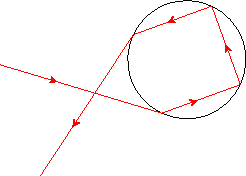
\includegraphics[scale=1]{arcsurnum}
		\caption{Schéma de principe de réflexions conduisant à un arc surnuméraire.
			\protect \pt{1} + \protect \pt{1}}
		\label{fig:arcsurnum}
	\end{figure}
}%

\end{document}%
